\documentclass[12pt,a4paper]{article}
\usepackage[UTF8]{ctex}
\usepackage{amsmath}
\usepackage{graphicx}
\usepackage{booktabs}
\usepackage{geometry}
\usepackage{ulem}
\geometry{left=2.5cm,right=2.5cm,top=2.5cm,bottom=2.5cm}

\title{\Huge{\textbf{\uuline{实\ 验\ 报\ 告}}}}
\author{\uline{少年班学院} \quad 姓名: \uline{李大恕} \quad 学号: \uline{PB24000145} \quad 实验日期: \uline{2025--4--21}}
\date{\today}

\begin{document}

\maketitle

\section{实验题目}
	衍射实验

\section{实验目的}
    \begin{enumerate}
        \item 对光学实验形成感性的认知，掌握组装、调整衍射实验光路的方法；
        \item 使用不同结构衍射屏实现夫琅禾费衍射，观察实验现象，研究不同结构衍射屏的衍射光强分布特征；
        \item 结合理论计算衍射屏的结构参数，包括单缝的缝宽 双缝中心间距以及小孔的直径。
    \end{enumerate}

\section{实验原理}
    \subsection{衍射现象概述}
    当波在传播过程中遇到尺寸与波长相当的障碍物或缝隙时，会发生绕射——波从几何光学的直线传播偏离，绕过边缘继续向前。这种现象最早由 Grimaldi 发现，并由惠更斯–菲涅尔原理加以解释：可把障碍物处的每一点都看作次级波源，子波在观察屏上相干叠加形成明暗条纹。

    \subsection{夫琅禾费衍射条件}
        \textbf{定义}：当光源和观察屏都位于衍射元件的“远场”位置（或通过透镜将光源、屏幕分别置于焦平面），入射光与衍射光均可近似看作平行光，此时的衍射称为夫琅禾费衍射。

        \textbf{优点}：图样稳定、结构简单，便于用数学方法精确计算各级明暗条纹的位置与强度。

    \subsection{单缝夫琅禾费衍射}
        \begin{enumerate}
            \item \textbf{物理模型}：用宽度为$a$的狭缝截取一束平行单色光（波长$\lambda$），在足够远的屏上观察其衍射图样。
                \begin{center}
                    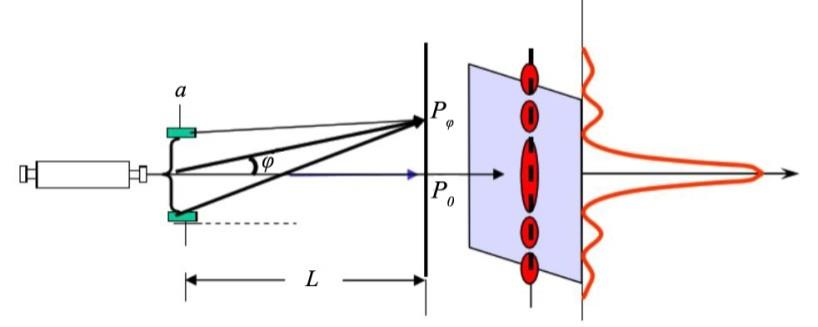
\includegraphics[width=0.5\textwidth]{简化单缝夫琅禾费衍射光路图.jpg} \\
                    \textbf{图1：单缝衍射光路图}
                \end{center}
            \item \textbf{光强分布}：沿屏面某点与光轴所成夹角$\varphi$，其光强
                \[
                    I(\varphi)=I_0\left(\frac{\sin u}{u}\right)^2,\quad u=\frac{\pi a\sin\varphi}{\lambda}
                \]
                \begin{center}
                    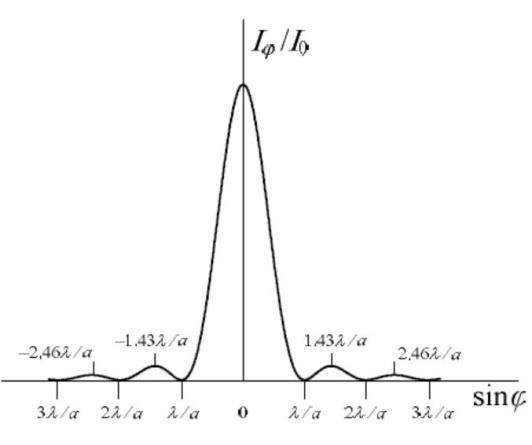
\includegraphics[width=0.5\textwidth]{单缝衍射相对光强分布曲线.jpg} \\
                    \textbf{图2：单缝衍射光强分布}
                \end{center}
            \item \textbf{暗纹与亮纹位置}：
                \begin{itemize}
                    \item 暗纹位置：$a\sin\varphi=k\lambda\quad(k=0,\pm1,\pm2,\cdots)$
                    \item 中央亮纹最宽、最亮，其两侧暗纹之间呈等间距分布；次级亮纹强度按衰减规律依次减小。
                \end{itemize}
        \end{enumerate}

    \subsection{双缝夫琅禾费衍射}
        \begin{enumerate}
            \item \textbf{物理模型}：两条等宽狭缝（宽度$a$），间距（中心到中心为$d$，共同接受平行单色光。
                \begin{center}
                    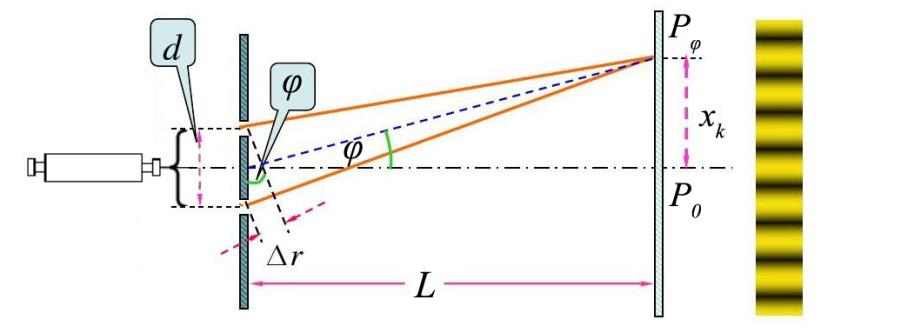
\includegraphics[width=0.5\textwidth]{双缝衍射光路图.jpg} \\
                    \textbf{图3：双缝衍射光路图}
                \end{center}
            \item \textbf{光强分布}：
                \[
                    I(\varphi)=I_0\left(\frac{\sin u}{u}\right)^2\cos^2 v,\quad u=\frac{\pi a\sin\varphi}{\lambda},\, v=\frac{\pi d\sin\varphi}{\lambda}
                \]
            \item \textbf{干涉极大/极小}：
                \begin{itemize}
                    \item 干涉极大：$d\sin\varphi=k\lambda\quad(k=0,\pm1,\pm2,\cdots)$
                    \item 干涉极小：$d\sin\varphi=(k+\frac{1}{2})\lambda\quad(k=0,\pm1,\pm2,\cdots)$
                    \item 当干涉极大与单缝衍射极小重合时，会出现缺级现象。
                \end{itemize}
        \end{enumerate}

    \subsection{圆孔夫琅禾费衍射}
        \begin{enumerate}
            \item \textbf{物理模型}：光通过直径为$d$的圆孔后，在远场形成同心明暗环。
                \begin{center}
                    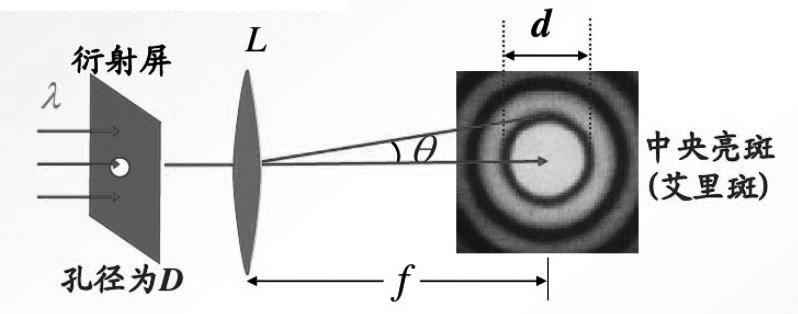
\includegraphics[width=0.5\textwidth]{圆孔夫琅禾费衍射.jpg} \\
                    \textbf{图4：圆孔衍射光路图}
                \end{center}
            \item \textbf{光强分布}：
                \[
                    I(\varphi)=I_0\left(\frac{2J_1(v)}{v}\right)^2,\quad v=\frac{\pi d\sin\varphi}{\lambda},\, J_1(v)=\frac{\sin v}{v}-\cos v
                \]
            \item \textbf{艾里斑}：第一暗环角满足
                \[
                    \sin\theta=\frac{1.22\lambda}{d}\approx\theta\quad(\theta\ll1)
                \]
            \item \textbf{应用}：在光学成像系统中，艾里斑大小决定系统的分辨极限。
        \end{enumerate}

\section{实验器材}
    \begin{itemize}
        \item He-Ne激光器（632.8nm）及电源
        \item 衍射元件：单缝，双缝，圆孔，弹簧等
        \item 光学导轨及附件：光学导轨，支架，一维平移台
        \item CCD，显示屏
    \end{itemize}

\section{基础实验}
    \subsection{实验步骤}
        \begin{enumerate}
            \item 观察单缝、双缝和小孔的衍射光强分布，总结各元件衍射图样的特点；
            \item 观察并总结单缝、双缝和小孔缝宽（或直径）变化时衍射图样的变化规律。
        \end{enumerate}
        
    \subsection{实验现象}
        \begin{enumerate}
            \item 单缝衍射图样：中央亮纹最宽、最亮，次级亮纹强度依次减小；单缝越宽条纹间距越小；
            \item 双缝衍射图样：条纹亮度振荡衰减；双缝间距越大条纹越窄；
            \item 小孔衍射图样：中央有艾里斑，环形条纹，亮度逐级衰减；孔直径越大艾里斑越小。
        \end{enumerate}
    

\section{提升实验}
    \subsection{实验步骤}
        \begin{enumerate}
            \item 记录单缝衍射各级暗条纹和中央主极大位置，计算单缝缝宽$a$，求相对误差；
            \item 记录双缝衍射各级亮条纹（或暗条纹）位置，计算双缝中心间距$d$，求相对误差。\\
                （$d=a+b$，为光栅常数，即其空间周期，$a$为缝宽，$b$为不透光部分的宽度）            
        \end{enumerate}

    \subsection{单缝衍射}
        \subsubsection{原始数据}
            \begin{center}
                \begin{tabular}{cccccccc}
                    \toprule
                    级数 & -6 & -5 & -4 & -3 & -2 & -1 & 0 \\
                    \midrule
                    $x_k$ (mm) & 13.286 & 13.665 & 14.045 & 14.482 & 14.865 & 15.301 & 15.681 \\
                    \bottomrule
                \end{tabular} \\
                \begin{tabular}{ccccccc}
                    \toprule
                    级数 & 1 & 2 & 3 & 4 & 5 & 6 \\
                    \midrule
                    $x_k$ (mm) & 16.701 & 16.483 & 16.884 & 17.299 & 17.682 & 18.086 \\
                    \bottomrule
                \end{tabular} \\
                \textbf{表1：单缝衍射各级暗条纹位置} \\
            \end{center}
            选取单缝宽度：$200\,\mathrm{\mu m}$

        \subsubsection{数据处理}
            采用最小二乘法线性拟合$x_k$与级数的关系，如图所示：
            \begin{center}
                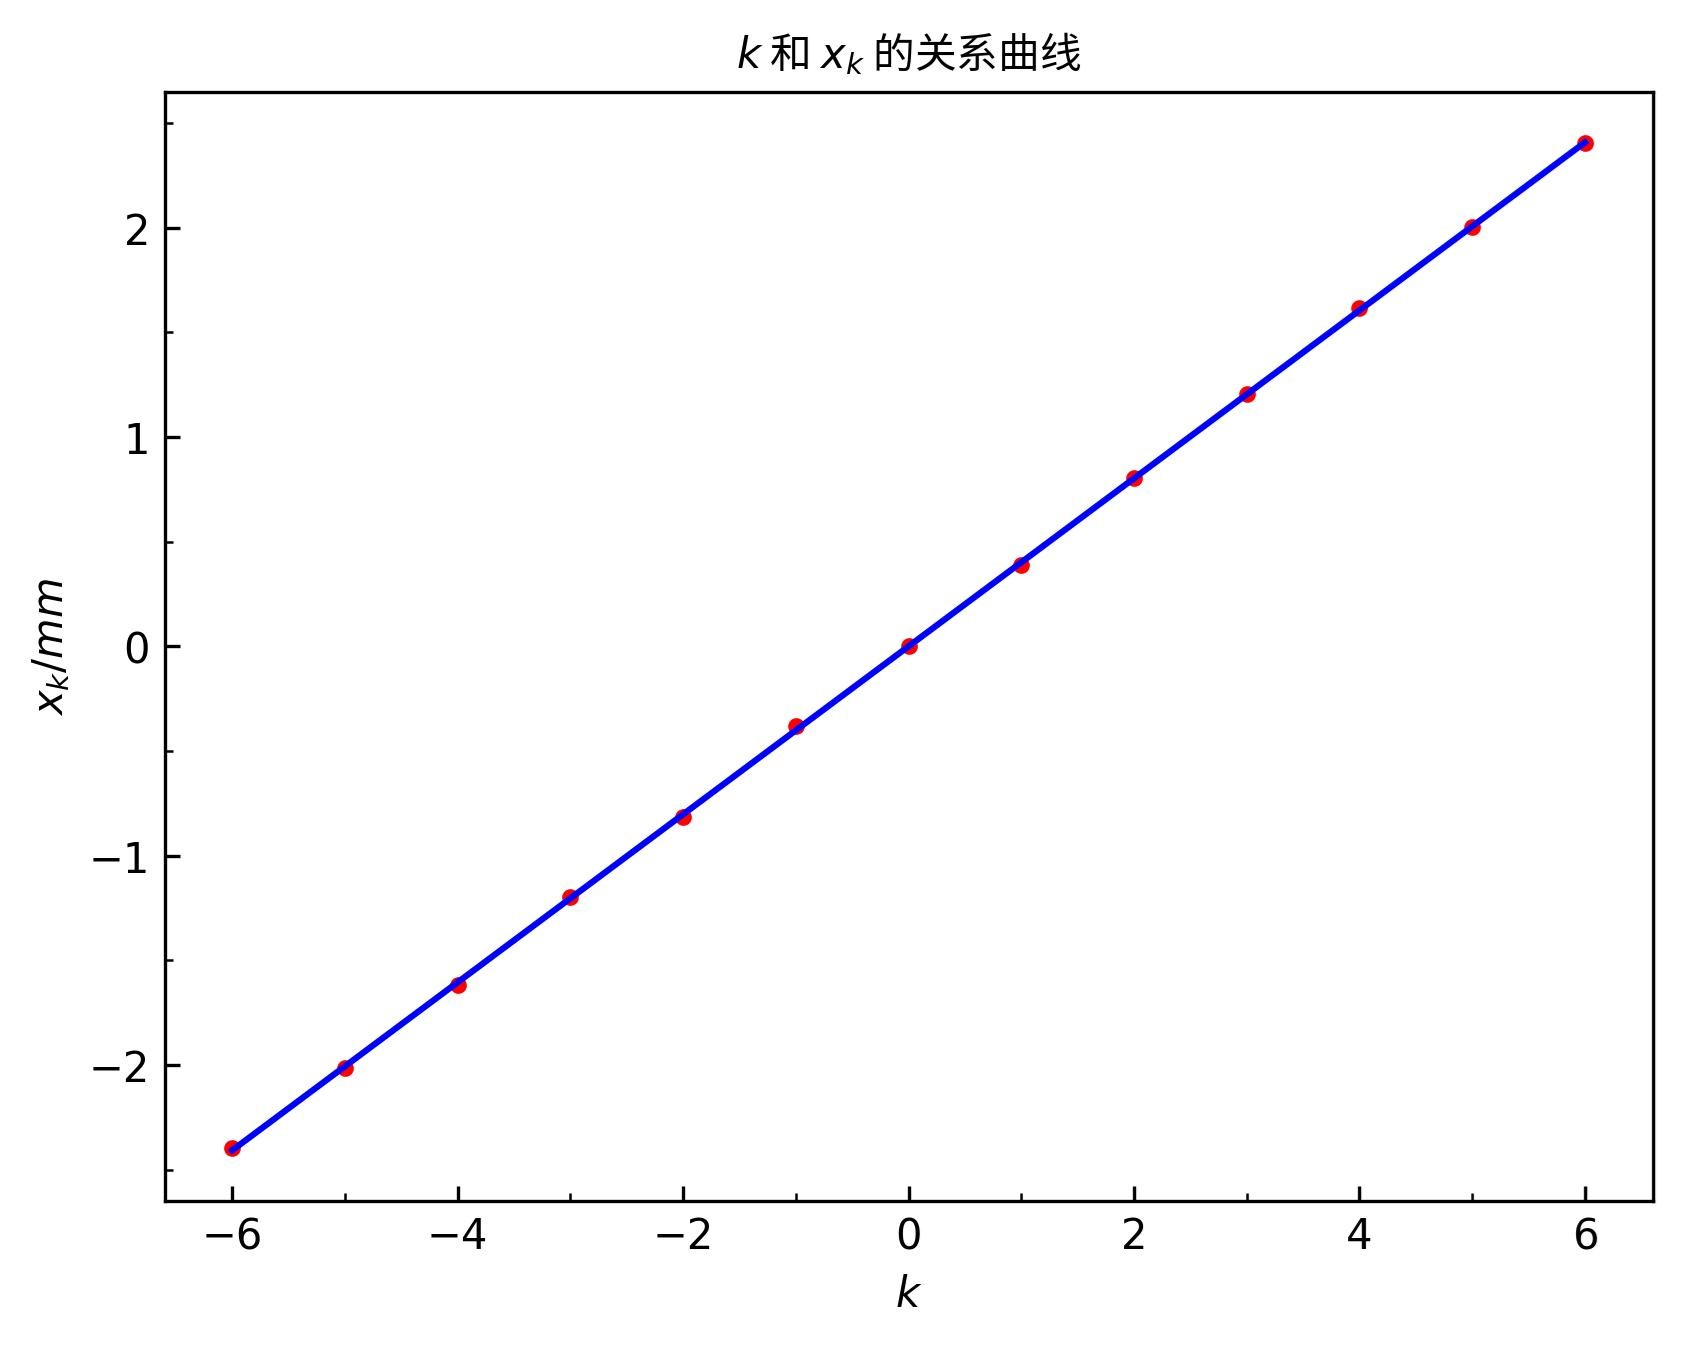
\includegraphics[width=0.8\textwidth]{单缝衍射线性拟合.jpg} \\
                \textbf{图5：单缝衍射线性拟合}
            \end{center}

            斜率
            \[
                m=0.40128\,\mathrm{mm}
            \]
            测得缝宽
            \[
                a=\frac{L \lambda }{m}=184.66\,\mathrm{mm}
            \]
            相对误差
            \[
                b=\frac{100 \left(- a + d\right)}{d}=\frac{100 \left(-184.66+200\right)}{200}\,\mathrm{\% }=7.6694\,\mathrm{\% }
            \]
    
    \subsection{双缝衍射}
        \subsubsection{原始数据}
            \begin{center}
                \begin{tabular}{cccccccc}
                    \toprule
                    级数 & -6 & -5 & -4 & -3 & -2 & -1 & 0 \\
                    \midrule
                    $x_k$ (mm) & 13.416 & 13.764 & 14.248 & 14.625 & 15.141 & 15.518 & 15.974 \\
                    \bottomrule
                \end{tabular} \\
                [1em]
                \begin{tabular}{ccccccc}
                    \toprule
                    级数 & 1 & 2 & 3 & 4 & 5 & 6 \\
                    \midrule
                    $x_k$ (mm) & 16.363 & 16.735 & 16.252 & 17.620 & 17.993 & 18.474 \\

                    \bottomrule
                \end{tabular} \\
                \textbf{表2：双缝衍射各级亮条纹位置} \\
            \end{center}
            选取双缝间距：$190\,\mathrm{\mu m}$

            \subsubsection{数据处理}
                同样采用最小二乘法线性拟合$x_k$与级数的关系，如图所示：
                \begin{center}
                    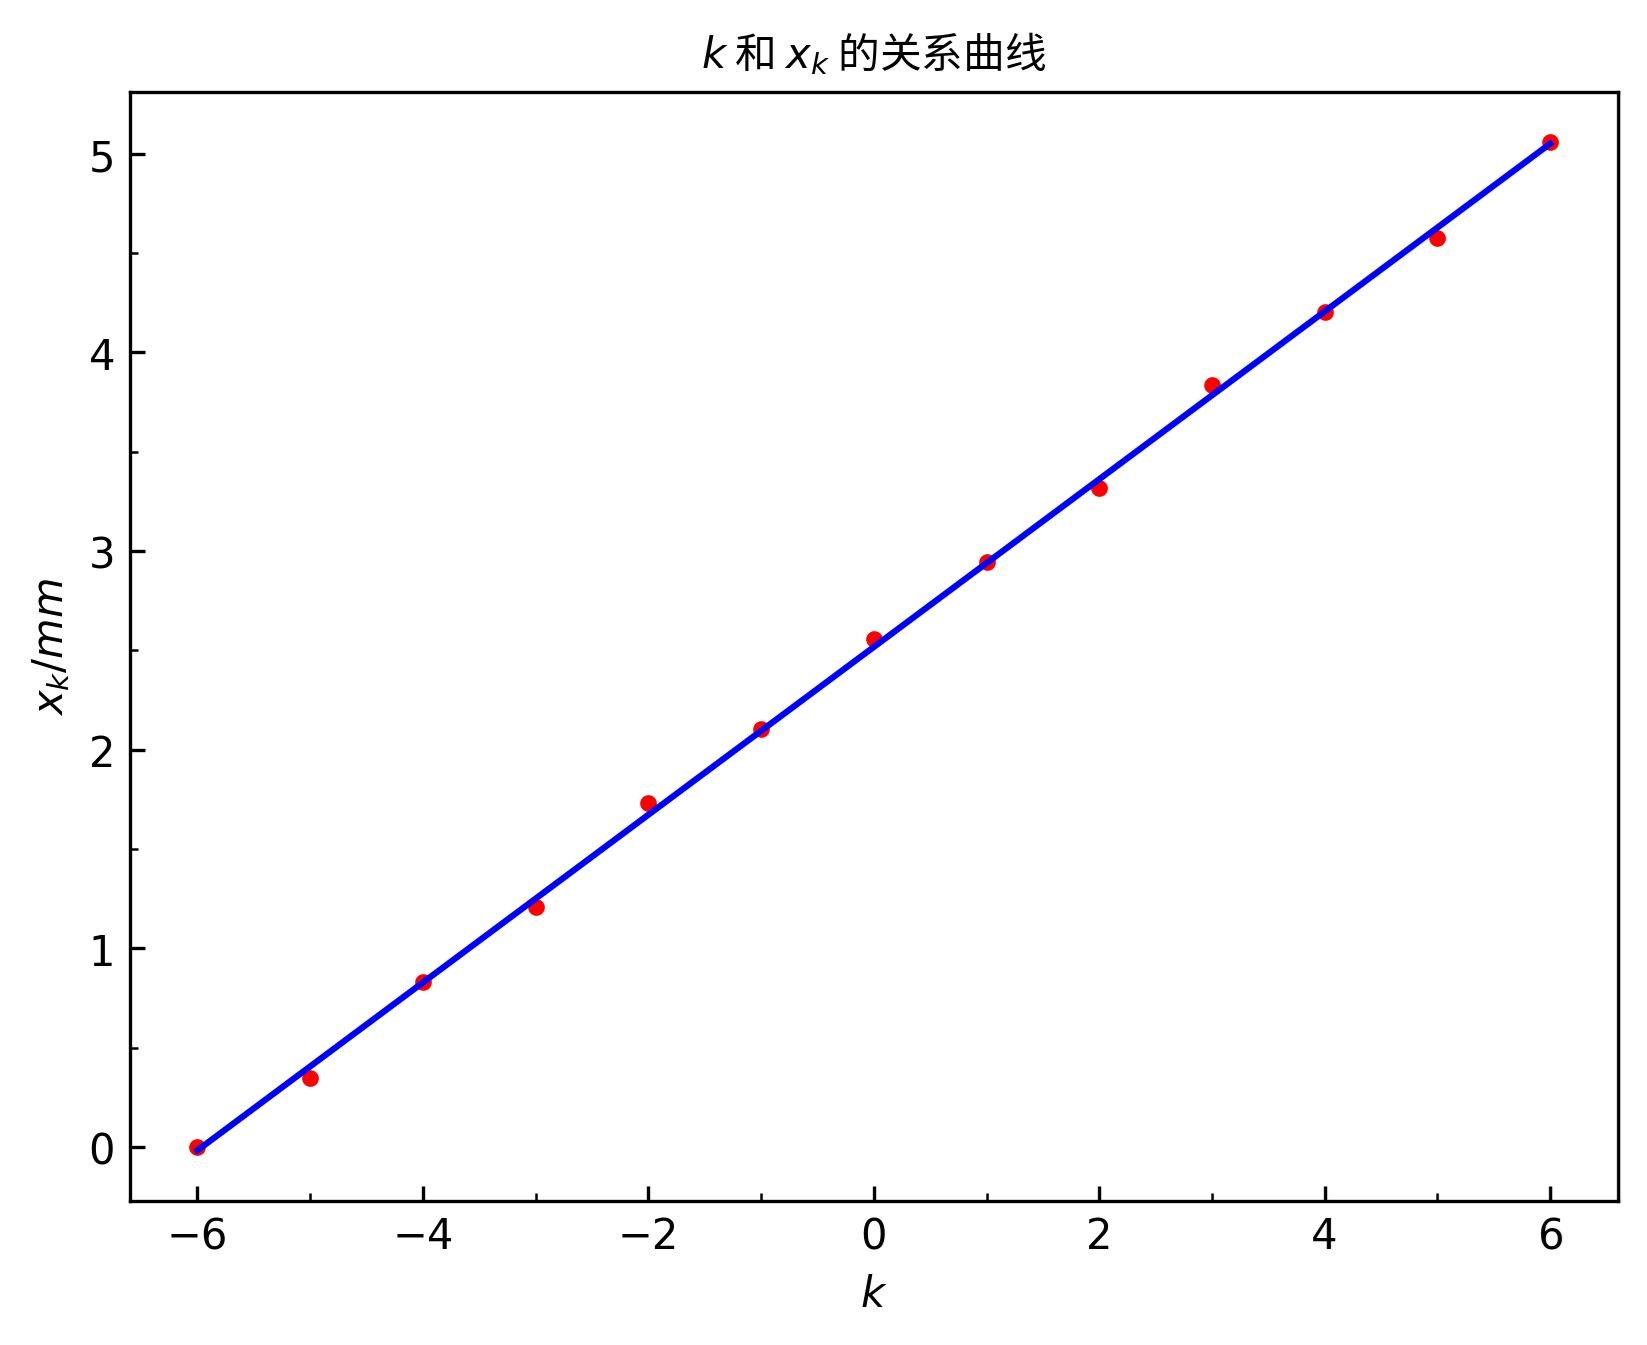
\includegraphics[width=0.8\textwidth]{双缝衍射线性拟合.jpg} \\
                    \textbf{图6：双缝衍射线性拟合}
                \end{center}

                斜率
                \[
                    m=0.42245\,\mathrm{mm}
                \]
                测得间距
                \[
                    a=\frac{L \lambda }{m}=175.41\,\mathrm{mm}
                \]
                相对误差
                \[
                    b=\frac{100 \left(- a + d\right)}{d}=\frac{100 \left(-175.41+190\right)}{190}\,\mathrm{\% }=7.6792\,\mathrm{\% }
                \]

            
\section{高阶实验}
    \subsection{实验目的}
        通过观察弹簧的衍射图样，计算弹簧的细丝直径和螺距。
    \subsection{实验步骤}
        \begin{enumerate}
            \item 观察弹簧的衍射图样，记录暗条纹位置；
            \item 计算弹簧的细丝直径和螺距。
        \end{enumerate}
    \subsection{原始数据}
        \begin{itemize}
            \item 距离$L=356.8\,\mathrm{cm}$
            \item 较宽暗条纹宽度$x=23\,\mathrm{mm}$
            \item 较窄暗条纹宽度$x=6\,\mathrm{mm}$
        \end{itemize}
        \begin{center}
            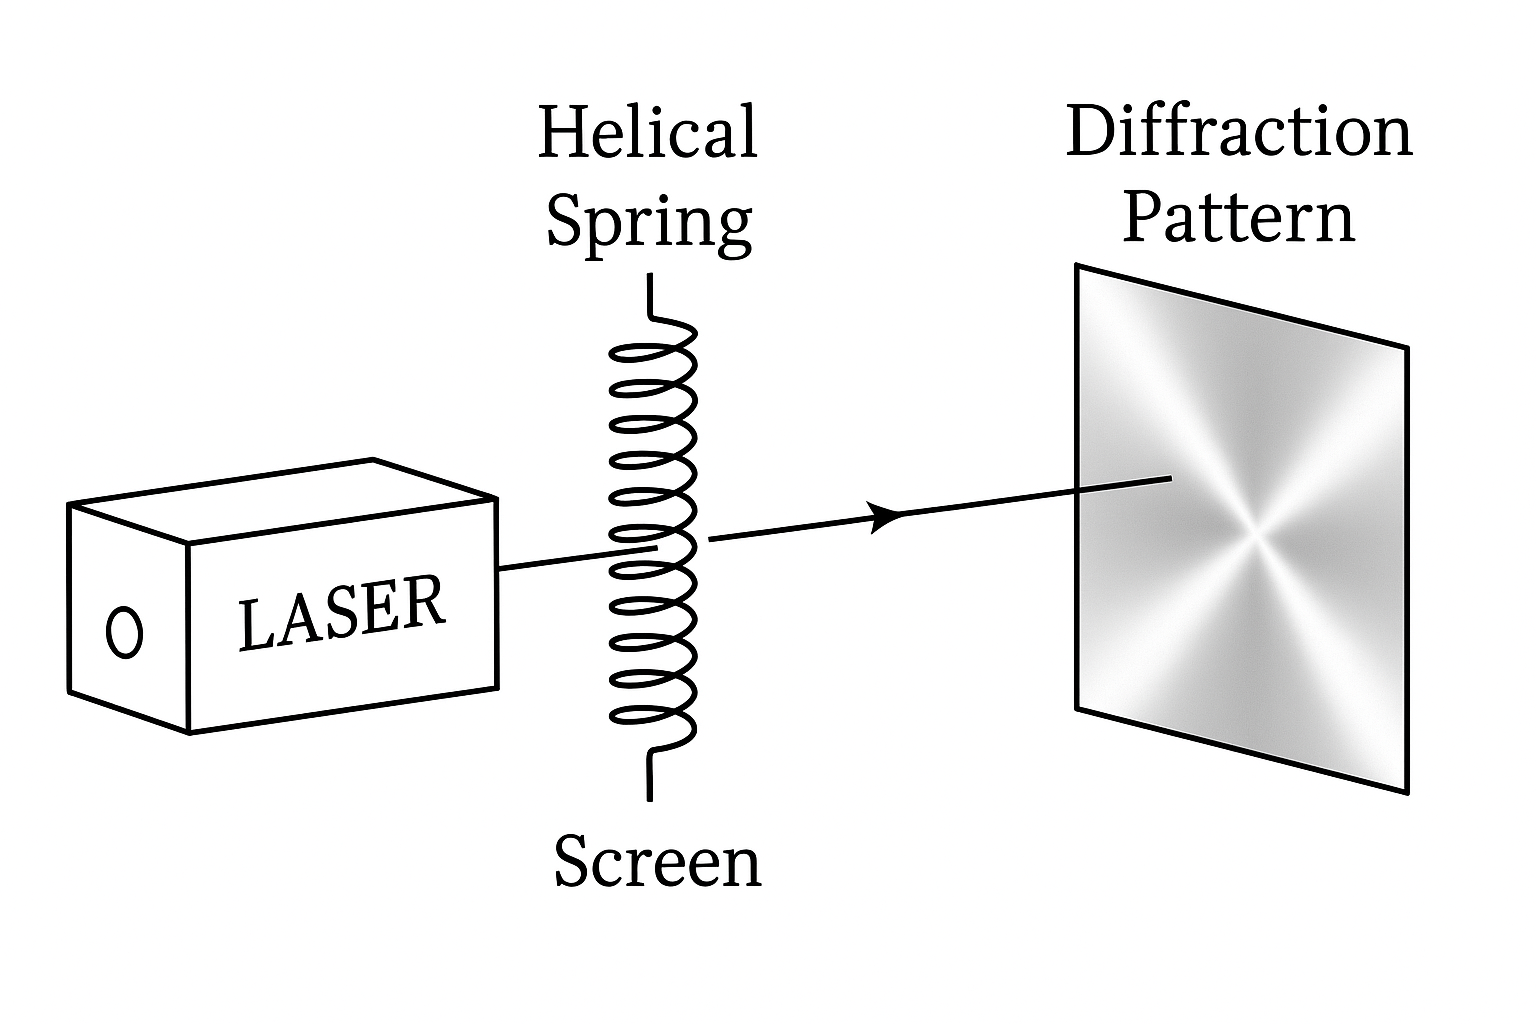
\includegraphics[width=0.8\textwidth]{弹簧衍射光路图.png} \\
            \textbf{图7：弹簧衍射光路图}
        \end{center}
    \subsection{参数计算}
        弹簧可看作光栅衍射。由光栅方程
        \[
            d\sin\varphi=k\lambda
        \]
        可得
        \[
            d=\frac{L \lambda }{x}
        \]
        其中$L$为光栅到屏幕的距离，$\lambda$为光源波长，$x$为暗条纹间距。
        
        由此可得，弹簧细丝直径
        \[
            d_{1}=\frac{L \lambda }{x}=98.167\,\mathrm{\mu m}
        \]
        弹簧螺距
        \[
            d_{2}=\frac{L \lambda }{y}=376.31\,\mathrm{\mu m}
        \]


\section{误差分析}
    \subsection{测量误差}
        \begin{itemize}
            \item \textbf{条纹位置读数误差}：条纹边缘不够清晰或亮暗对比不强，使得用千分尺测量条纹中心位置时存在估读误差；
            \item \textbf{重复性差异}：人为判断不同级条纹位置存在主观偏差，特别是在中央以外的次级条纹处；
            \item \textbf{单一测量值}：某些数据如$L$、$x$、$y$等只有单组数据。
        \end{itemize}
    \subsection{仪器误差}
        \begin{itemize}
            \item \textbf{平移台精度限制}：螺旋测微器、CCD 位移装置等本身存在系统误差或分辨率限制；
            \item \textbf{激光器发散角度}：虽然理论上是准直光，但激光发散或调节误差会造成衍射角偏移；
            \item \textbf{CCD灵敏度}：图像中像素的响应精度及对比度处理方式可能引入条纹提取误差。
        \end{itemize}
    \subsection{理论简化引入的误差}
        \begin{itemize}
            \item \textbf{小角近似$(\sin\varphi\approx\varphi)$}：只在衍射角较小时成立，条纹级数过高可能造成理论偏离；
            \item \textbf{假设光为理想平行光}：实际光束略有发散，远未达到理论“无穷远”条件；
        \end{itemize}


\section{思考题}
    \begin{enumerate}
        \item \textbf{当光通过一个小孔时，在后面的光屏上会得到什么样的图案？} \\
            当光通过一个小孔时，在远处的屏幕上将形成一个以艾里斑为主的圆形衍射图样。该图样的主要特征为：中央是一个强度最大的亮斑，称为中央主极大；周围是多个亮暗交替的同心圆环，亮度逐渐减弱；明暗条纹的间距随小孔直径减小而增大。
        \item \textbf{白光照射到狭缝上，衍射条纹有什么特点？} \\
            白光由多种波长的单色光组成，因此当其照射到狭缝上时，不同波长的光会产生不同的衍射角，导致条纹具有如下特点：中央亮纹为白色，因为各色光在此位置重合；离中心越远的条纹越呈现彩色分布，不同波长的光分别在不同位置达到干涉条件；条纹呈现彩虹状、带色彩分离的效果，是衍射中的色散现象。这说明白光衍射条纹不仅有强度分布，还有波长分离的现象，进一步验证了光的波动和多色特性。
        \item \textbf{蝴蝶翅膀的颜色和图案会随观测角度的变化而发生改变，讨论产生这种现象的原因。} \\
            蝴蝶翅膀颜色随观察角度变化的现象被称为结构色现象。其本质原因是翅膀表面存在规则排列的微纳米结构，这些结构对光产生以下影响：光在翅膀的微结构中发生干涉和衍射；不同角度下，不同波长的光满足干涉增强条件，从而显示不同颜色；颜色的变化是由微结构与光的相互作用决定的光学效应，是光波干涉与衍射的综合表现。
    \end{enumerate}

\appendix
    \section{老师签字的原始数据}
        \begin{center}
            
\includegraphics[width=0.8\textwidth]{原始数据1.jpg} \\
            
\includegraphics[width=0.8\textwidth]{原始数据2.jpg}
        \end{center}

\end{document}
